\documentclass[]{article}
\usepackage[a4paper, total={6in, 8in}]{geometry}
\usepackage{booktabs}
\usepackage{multicol}
\usepackage[
  sorting=none,
  sortcites=true,
  backend=bibtex,
  giveninits=true,
  style=authoryear-comp,
  natbib=true,
  maxcitenames=2,
]{biblatex}
\bibliography{bibliography}

\newcommand{\todo}[1]{{\color{red}[\textit{TODO: #1}]}}

\usepackage{tikz}
\usetikzlibrary{calc}
\usetikzlibrary{shapes.geometric, arrows, fit}

\tikzstyle{process} = [rectangle, 
minimum width=12cm, 
minimum height=1cm, 
text width=11cm, 
draw=black, 
fill=white,
rounded corners]

\tikzstyle{subprocess} = [rectangle, 
minimum width=5cm, 
minimum height=0.6cm, 
text centered, 
text width=5cm, 
draw=black, 
fill=white]

\tikzstyle{lsnode} = [rectangle, 
minimum width=2cm, 
minimum height=0.6cm, 
text centered, 
text width=2cm, 
draw=black, 
fill=white]

\tikzstyle{arrow} = [thick,->,>=stealth]
\tikzstyle{dashedarrow} = [dashed,->,>=stealth]

\title{Integrated Vehicle and Crew Scheduling for Electric Buses using Lagrangian Relaxation}
\date{July 2025}
\author{Thomas van der Plas, Han Hoogeveen, Philip de Bruin}
\begin{document}
\maketitle

\section{Introduction}
\begin{figure}
  \centering
  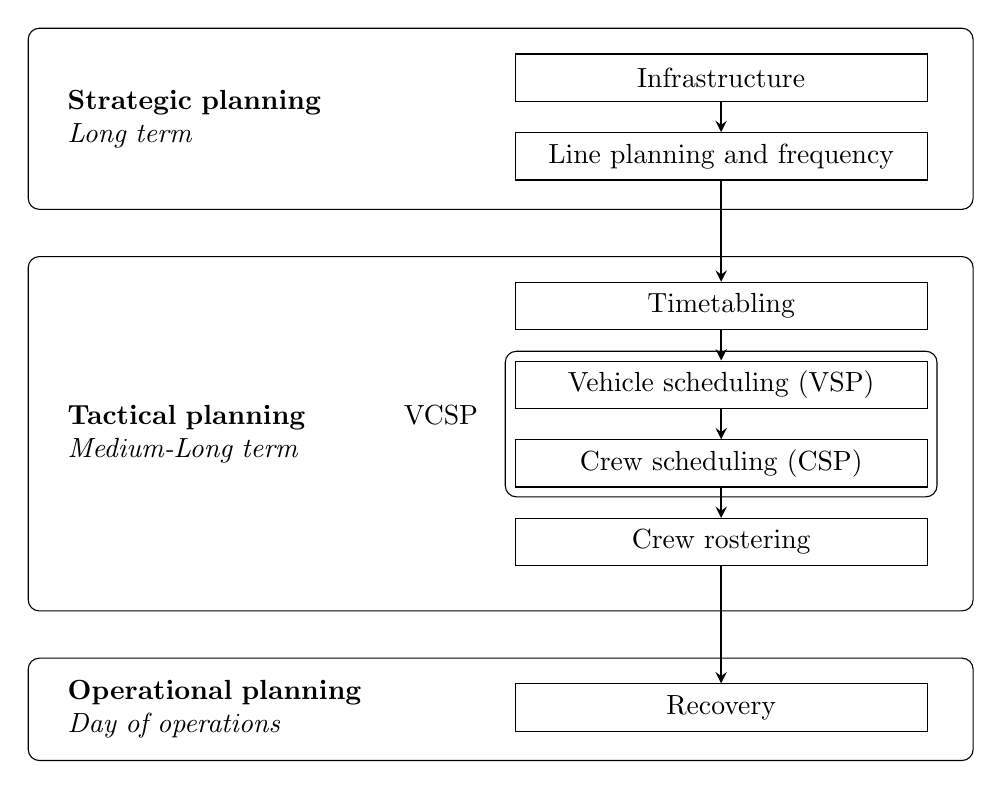
\begin{tikzpicture}[node distance=2cm]
    \node (strategic) [process, minimum height=2.3cm] {\textbf{Strategic planning}\\\textit{Long term}};
    \node at (strategic.base) (infra) [subprocess, xshift=2.8cm, yshift=0.4cm] {Infrastructure};
    \node at (strategic.base) (line) [subprocess, below of=infra, yshift=1cm] {Line planning and frequency};

    \node (tactical) [process, minimum height=4.5cm, below of=strategic, yshift=-2cm] {\textbf{Tactical planning}\\\textit{Medium-Long term}};
    \node at (tactical.base) (timetable) [subprocess, xshift=2.8cm, yshift=1.5cm] {Timetabling};
    \node at (tactical.base) (vehicle) [subprocess, below of=timetable, yshift=1cm] {Vehicle scheduling (VSP)};
    \node at (tactical.base) (crew) [subprocess, below of=vehicle, yshift=1cm] {Crew scheduling (CSP)};
    \node at (tactical.base) (VCSP) [rounded corners, draw=black, fit=(vehicle) (crew), align=left] {\hspace{-4em}VCSP};
    \node at (tactical.base) (rostering) [subprocess, below of=crew, yshift=1cm] {Crew rostering};

    \node (operational) [process, minimum height=1.3cm, below of=tactical, yshift=-1.5cm] {\textbf{Operational planning}\\\textit{Day of operations}};
    \node at (operational.base) (recovery) [subprocess, xshift=2.8cm, yshift=-0.1cm] {Recovery};

    \draw [arrow] (infra) -- (line);
    \draw [arrow] (line) -- (timetable);
    \draw [arrow] (timetable) -- (vehicle);
    \draw [arrow] (vehicle) -- (crew);
    \draw [arrow] (crew) -- (rostering);
    \draw [arrow] (rostering) -- (recovery);
  \end{tikzpicture}
  \caption{A general overview of the public transport planning process, based on \citet{Ceder1986, Ibarra-Rojas2015, Perumal2022LitRev}.}
  \label{fig:planning-overview}
\end{figure}
Electric vehicles are beginning to make up large portions of the fleet for
public transport providers. In The Netherlands for instance, around 21\% of all
registered buses are already electric according to the \citet{RDW}. However,
in order to meet \citet{europaRegulation20181999} on climate and sustainability, individual
line operators such as the Dutch \citet{qbuzzQbuzz} are slowly replacing even more of their old
combustion based fleet with electric vehicles. It is therefore almost certain that this share will only grow in
coming years across different countries. \\
This shift in energy source has introduced new challenges to the methods currently in use to keep our public transport moving. Of primary concern are charging infrastructure and vehicle ranges, both of which are much more limited than their traditional combustion based counterparts. The planning process which has traditionally been used, as outlined in Figure \ref{fig:planning-overview}, therefore requires additional research into each of its steps in order to incorporate these newly relevant constraints.\\
\noindent In this work, we will focus on incorporating electric vehicle restrictions into two of these steps: vehicle scheduling and crew scheduling. Specifically, we will consider the scheduling of electric buses and their drivers, as these two steps make up a majority of day-to-day costs within the bus transit sector. \\
The goal of vehicle scheduling (also referred to as the vehicle scheduling problem or VSP) is to find a minimum cost schedule for vehicles in order to cover a set of predetermined trips. In the case of buses our trips are given by a timetable for each individual route, which is the result of the previous step of the planning process. Using the trips defined in such a timetable, our goal is therefore to assign sequences of compatible trips to buses such that each individual trip is driven. \\
In order to do this, a collection of vehicle tasks must be generated. A vehicle task can be seen as the individual schedule that a bus will follow throughout the day: it may start at a bus storage facility (more commonly called a depot), then perform one or more trips, before finally returning to the depot. The driving actions performed between between a depot and a trip, as well as those between trips themselves are called deadheads. The costs of driven deadheads along with the total number of buses used are the main focus for minimization, as the costs incurred for driving the trips themselves is fixed. \\
Once vehicle schedules are known, we can move on to the crew scheduling problem (CSP). Here, our goal is to find minimum cost assignment of crew members to vehicles. Continuing within the context of bus planning, we now need to match drivers with our previously planned buses. Driving time for a driver is often limited in a single day, and for longer shifts breaks might be mandatory as well; it is therefore not always possible to create a one to one matching between crew and vehicle tasks. It is therefore necessary to split vehicle tasks up into multiple segments, whereafter we can create crew tasks that consist of one or more compatible segments. As before with the trips, the vehicle tasks themselves are fixed; in order to minimize costs, we must find a covering set of crew tasks which minimizes the number of required crew members and unused paid hours. \\ 
Crew scheduling is the greatest contributor to day-to-day costs; a recent estimate by \citet{Perumal2019Crew} puts it at around 60\% of the overall operational costs for bus transit providers in Northern Europe. As can be seen however, the VSP and CSP are very closely related. The vehicle tasks that are selected in the VSP directly determine what crew
tasks are feasible within the CSP. It is therefore not always optimal to
fully minimize costs in the vehicle scheduling process, as this might incur
higher overall costs due to crew scheduling. We can therefore roughly split the
solving of vehicle and crew assignments into two separate approaches:
sequential, in which the VSP and CSP are solved separately, or integrated, in
which the VSP and CSP are solved such that overall costs are minimized
simultaneously. The integrated approach is often referred to as the vehicle and
crew scheduling problem, or VCSP. \\
A lot of work has already been done for the VSP, CSP and VCSP.
Both the sequential and integrated approach have been extensively studied since the 1980s, as shown by surveys such as \citet{Bodin1983}. The introduction of electric vehicles has however introduced significant constraints on charging and vehicle ranges, invalidating a formerly often made assumption that a vehicle was able to drive an entire day without being refueled. This most directly effects the VSP, as charging periods now need to be added throughout the day in order to
effectively use buses. The version of the vehicle scheduling problem which incorporates these constraints, referred to as the
E-VSP, has been the focus of many studies going back to around 2014. We refer the reader
to a survey by Perumal et al. for a detailed overview of recent progress
\citet{Perumal2022LitRev}. \\
Limited literature does exist on the integrated VCSP with electric vehicles (E-VCSP), however
simplifying assumptions are made which might limit real world applicability or
accurate modeling of costs. Most notably, assumptions are currently made about charging
locations (such as only being able to charge at a bus depot) or charging
behavior (such as modeling the process as being purely linear or only allowing
full charges). Additionally, to the best of our knowledge battery degradation
due to usage patterns has not been included in any integrated models at the
time of writing. Our aim is to introduce a model which incorporates more realistic behavior for battery charging and usage, by including the following:
\begin{itemize}
  \item Including nonlinear battery charging times.
  \item Considering the cost of battery degradation due to usage patterns.
  \item Allowing for capacitated charging stations at both depots and the endpoints of a trip.
  \item Allowing partial charging of the battery throughout the day.
\end{itemize}
This work is organized as follows. In Section 2, we will discuss work related to the E-VCSP and give an overview of common ways of modeling and solving the problem. In Section 3, we give our formal problem definition.\ \todo{Meer secties}.

% We will now give an informal overview of the
% problems at hand. A more formal definition can be found in Section
% \ref{sec:problem_def} \todo{work in progress}. \\
% The Vehicle Scheduling Problem (VSP) aims to find a set
% of minimum cost vehicle tasks such that all trips that need to be driven
% throughout a time period are covered. In this, a trip is defined as full or
% partial travel of a vehicle along a predetermined route, and a vehicle task is
% defined as a set of sequential operations that a vehicle will perform. A task for a
% vehicle must start at a depot, perform a number of compatible trips (that is,
% trips which can be performed sequentially while respecting driving times
% between trips), before finally returning to its original depot. In order to
% minimize operational costs, both the number of used vehicles and the overall driven
% distance between trips need to be minimized. \\ The VSP
% with a single depot and unconstrained vehicle ranges can be solved in
% polynomial time \citet{Freling2003SDVSP}. The multi-depot variant of the problem
% on the other hand is known to be NP-hard, and the addition of constrained vehicle ranges such as those found
% in EVs also make the problem NP-hard \citet{Bodin1983}. We will consider a
% general depot case with constrained vehicle ranges due to the inclusion of EVs,
% and will therefore refer to the VSP as being NP-Hard. \\\\ The Crew
% Scheduling Problem (CSP) on the other hand aims to find a minimum cost
% assignment of crew members to vehicle tasks. Given a set of vehicle tasks and
% crew members, the goal is to find an assignment of crew members such that each
% vehicle is always driven by at least one driver. In this, constraints such as
% maximum working time on a day, driver breaks and handovers between different
% drivers on the same vehicle need to be considered. The primary goal for
% minimization here is the total number of workers needed and hours worked. The
% CSP is also known to be an NP-hard problem \citet{Fischetti1989}.\\\\ As can be seen, the VSP and CSP are closely related.  

\begin{table}[h]
  \centering
  \begin{tabular}{ll}
    \toprule
    \multicolumn{1}{l}{\textbf{Abbreviation}} & \multicolumn{1}{l}{\textbf{Definition}}               \\
    \cmidrule(lr){1-1}\cmidrule(lr){2-2}
    ALNS                                      & Adaptive Large Neighborhood Search                   \\
    B\&P                                      & Branch-and-Price                                      \\
    CG                                        & Column Generation                                     \\
    CP                                        & Constraint Programming                                \\
    CSP                                       & Crew Scheduling Problem                               \\
    E-\dots                                   & Problem \dots with electric vehicles                  \\
    LNS                                       & Large Neighborhood Search                            \\
    LS                                        & Local Search                                          \\
    MDVSP                                     & Multi Depot Vehicle Scheduling Problem                \\
    MIP                                       & Mixed Integer Program                                 \\
    SAA                                       & Simulated Annealing Algorithm                         \\
    SDVSP                                     & Single Depot Vehicle Scheduling Problem               \\
    SoC                                       & State of Charge                                       \\
    TCO                                       & Total Cost of Ownership                               \\
    ToU                                       & Time of Usage                                         \\
    TVSP                                      & Integrated Timetabling and Vehicle Scheduling Problem \\
    VCSP                                      & Integrated Vehicle and Crew Scheduling Problem        \\
    VSP                                       & Vehicle Scheduling Problem                            \\
    \bottomrule
  \end{tabular}
  \label{tab:nomenclature}
  \caption{Nomenclature used in this work}
\end{table}

\section{Related work}
In this section, we will discuss work related to our research into the E-VCSP. An overview of the nomenclature used has been included in Table \ref{tab:nomenclature}, and an summary of how batteries and charging behavior is modeled in the discussed works has been included in Table \ref{tab:eVCSP-lit}. \\\\
\begin{table}[]
  \centering
  \begin{tabular}{clllllll}
    \toprule
                                     & Model   & ToU & SoC & Nonlinear Ch. & Partial Ch. & Ch. Location & Degradation \\
    \cmidrule(lr){2-8}
    \citet{Li2014} 2014               & E-VSP   & No  & D   & No            & No          & D            & No          \\
    \citet{vanKootenNiekerk2017} 2017 & E-VSP   & Yes & C/D & Yes           & Yes         & D/T          & Yes         \\
    \citet{Olsen2020} 2020            & E-VSP   & No  & C   & Yes           & Yes         & D/T          & No          \\
    \citet{Zhang2021} 2021            & E-VSP   & No  & C/D & Yes           & Yes         & D            & Yes         \\
    \citet{Parmentier2023} 2023       & E-VSP   & No  & C   & Yes           & Yes         & D/T          & No          \\
    \citet{Pulyassary2024} 2024       & E-VSP   & No  & C/D & Yes           & Yes         & T            & No          \\
    \citet{deVos2024} 2024            & E-VSP   & No  & D   & Yes           & Yes         & D/T          & No          \\
    \addlinespace[0.4em]
    \citet{Perumal2021} 2021          & E-VCSP  & No  & C   & No            & No          & D            & No          \\
    \citet{Wang2022} 2022             & E-VCSP  & Yes & C   & No            & Yes         & D            & No          \\
    \citet{Sistig2023} 2023           & E-VCSP  & No  & C   & No            & Yes         & D/T          & No          \\
    \citet{Shen2023} 2023             & E-VCSP  & No  & C   & No            & No          & D/T          & No          \\
    \citet{Cong2024} 2024             & E-VCSP  & Yes & C   & No            & Yes         & D            & No          \\
    \addlinespace[0.4em]
    \citet{Ham2021} 2021              & E-VRPTW & Yes & C   & No            & Yes         & D            & No          \\
    \citet{Stadnichuk2024} 2024       & E-TVSP  & No  & C   & No            & Yes         & D/T          & No          \\
    \bottomrule
  \end{tabular}
  \caption{A brief overview of battery modeling in E-VCSP related literature. SoC modeled as (D)iscrete or (C)ontinuous variable, Charge locations at (D)epot or (T)erminal trip stops, Degradation of battery in cost function}
  \label{tab:eVCSP-lit}
\end{table}
\todo{uitleg van de SDVSP}
\noindent \textbf{(E-)VSP} \\
The SDVSP has long been known to be polynomially solvable, however the inclusion of
multiple depots has been shown to make the problem NP-hard under the assumption
that buses must return to the same depot from which they originated
\citet{Bunte2009}. Additionally, the introduction of any resource constraints
such as limited ranges within the VSP has also been shown to be NP-hard by
Bodin et al. \citet{Bodin1983}. As the E-VSP deals with the limited range
associated with electric vehicles, it is quite closely related to the multiple
depot vehicle scheduling problem with route time constraints (MDVSP-RTC)
\citet{Haghani2002}. The key difference between these two problems is that the
E-VSP allows for (partial) recharging of a vehicle throughout the operating
period, whereas the MDVSP-RTC assumes a fixed maximum travel time for the
vehicle within the given period. The E-VSP specifically been shown to be
NP-hard by Oulamara and Sassi \citet{Sassi2014}. \\\\
Li was one of the first to consider the E-VSP back in 2014 \citet{Li2014}. The
model is based on an extension of the traditional network based approach to
solving the VSP, with the additional constraint of total driving time. It
additionally assumes that fast charging or battery swaps are possible, ensuring
full charges in a fixed time span. The model is solved using a column generation
approach with branch-and-price, followed by a local search to find a local
optimum. The proposed methods are tested on trips in the San Francisco Bay
Area, with a maximum instance size of 242 trips. These tests resulted in
optimality gaps of $<5\%$ for buses able to drive 150km, and between 7-15\%
for a range of 120km depending on the instance. \\\\
Van Kooten Niekerk et al.\ introduce a two models which aim to solve the single depot E-VSP
while taking into account ToU energy prices, nonlinear charging times and
battery degradation due to depth of discharge \citet{vanKootenNiekerk2017}. The first model only allows for linear charging and no consideration for degradation or ToU, but uses continuous SoC variables. The second model does allow for the extra inclusions, at the cost of discretizing SoC and solving using CG for a possibly non-optimal solution. They test using data provided
by Belgian bus company De Lijn in the city Leuven, using a total of 543 trips. They show that the
discretized model can be solved in a considerably shorter time frame for large instances with similar results to
the continuous model. \\\\
\todo{langer!}
Olsen and Kliewer introduce a solution to the E-VSP which models the nonlinear phase of charging as an exponential function \citet{Olsen2020}. They focus on showing that a (piecewise) linear approximation for the second phase of charging can
misrepresent the SoC and required charging times. \\\\
Zhang et al. apply a similar method to the one found in van Kooten Niekerk
\citet{Zhang2021}. They consider a single depot with capacitated charging infrastructure,
with multiple round trip lines originating from the depot. They model
nonlinear charging behavior and battery depreciation due to depth of discharge using discretized time steps. They solve
using a combination of CG and B\&P. Tests are done on both randomly generated
instances as well as 6 not yet electrified lines with up to 160 and 197 trips
respectively.\\\\
\todo{beter formuleren}
Parmentier et al. consider a scalable approach to the E-VSP with non-linear charging~\citet{Parmentier2023}. They introduce the concept of nondominated charging arcs, which are defined as a deadhead arc between two trips during which charging is allowed with lower or equal cost and higher or equal resulting charge than all others deadhead arcs between the trips. In order to solve, a combination of CG and B\&P techniques are used. The nondominated charging arcs are used in order to formulate a more
computationally efficient version of the pricing problem given uniform charging
infrastructure. Testing is done on the \textit{large}
instances introduced by Wen et al. \citet{Wen2016} which included up to 8
depots, 16 charging stations and 500 trips. Here, they are able to find
solutions that only have an 0.06\% optimality gap. \\\\
\todo{Zoals Philip ook al zei laatst: deze paper komt van arxiv en is zover ik weet niet peer reviewed, maar leek me alsnog wel interessant.}Pulyassary et al. show that the single depot E-VSP is solvable in polynomial time given the
assumption that the shortest path between two trips in the flow network is
equal to the path with lowest battery usage \citet{Pulyassary2024}. They
consider the case in which charging at a select number of capacity bound nodes
is allowed with nonlinear charging behavior. For the single depot case, a
$O^*(|T|^6)$ algorithm for finding a set of vehicle schedules with lowest cost
given trips $T$ is provided based on DP. Additionally, polynomial algorithms
for determining maximum feasible charging capacity and minimum-cost flows based
on LP are provided. No computational experiments are performed. \\\\

\todo{beter schrijven}
De Vos et al. consider the E-VSP with partial recharges and capacitated charging stations \citet{deVos2024}. 
They model this using discrete SoC levels for each trip, as well as discrete time and SoC nodes for charging spots within the traditional network. This discretization is similar to that of van Kooten Niekerk et al., however now with the inclusion of capacitated charging nodes. Using this, a primal network is created using pessimistic
rounding. In order to solve, they apply CG with two separate approaches:
branch-and-price and a diving heuristic. To overcome the limitations of dual
bounds resulting from a discretized model, they incorporate ideas from Boland
et al. resulting in a dual network with optimistic connections
\citet{Boland2017}. This gives the same bounds as the ones found in the
non-discretized model. Testing is performed on a bus concession south of
Amsterdam with 816 trips, with subsets being used as smaller instances.
Optimality gaps of 1.5-2.7\% are achieved across instances. They additionally
note that the framework as provided can easily be extended for nonlinear
charging functions and depth-of-discharge battery degradation. \\\\

\noindent \textbf{CSP}\\
\todo{gegeven een oplossing voor de vsp}
Given a solution to the (E-)VSP, the corresponding CSP is most often solved as a set partitioning (or set covering) problem. Here, the tasks described by the sequences of trips generated during vehicle scheduling must be covered by the individual schedules of crew members. This problem has been shown to be NP-hard in general \citet{Fischetti1989}. Research into this subject is primarily done in the context of airline crew planning; crew costs in this field are generally even higher than those found in the more general public transport sector \citet{Barnhart2003}. Additionally, strong labor unions and restrictive labor legislation due to safety concerns cause a large number of constraints to be applied to crew schedules, resulting in a non-trivial problem to solve. \\
Results achieved in the aviation space quite easily generalize to other sectors, and we therefore refer the reader to a recent review by Deveci and Demirel for an overview of the state of the art \citet{Deveci2018}. \\\\

\noindent \textbf{(E-)VCSP}\\
The VCSP has been a widely studied problem. Following the call for integrated methods by Bodin et al. and others in the 1980s, a large number of different methods has been applied to integrate the VSP and CSP \citet{Bodin1983}. We refer the reader to a recent review for a more general overview of work done in the field in the past years \citet{Ge2024}. \\\\
One work that we will individually highlight is that of Huisman et al., due to its use of Lagrangian relaxation to connect the VSP and CSP \citet{Huisman2005}. For readers unfamiliar with the technique, we recommend an introduction by Beasley \citet{Beasley1993}. Huisman et al. consider the multi-depot variant, and use a combination of CG and Lagrangian relaxation to solve both the MDVSP as well as the connection with the CSP. Of note is their assumption that crew members from each individual depot are only allowed to work on trips connected to said depot, allowing for individual depot CSPs to be solved as a subproblem. They test on instances in the Randstad metro area in the Netherlands with a maximum of 653 trips and 4 depots. \\\\
As for the electric counterpart of the VCSP, at time of writing we are aware of only five other works that discuss the integrated variant. \\\\
Perumal et al. were the first to offer a solution to the E-VCSP in 2021
\citet{Perumal2021}. They introduced an ALNS which incorporates a B\&P heuristic
which has been previously used to solve the MDVSP, E-VSP and VCSP
\citet{Pepin2009, Haase1996, vanKootenNiekerk2017}. They only consider full recharges with a fixed duration of
120 minutes and charging at the depot. The
authors tested using real life data from lines in Denmark and Sweden with a
maximum instance size of 1109 trips and multiple depots, and report an improvement of $1.17-4.37\%$
across different instances when compared to a sequential approach. \\\\

Wang et al. introduce a two layered model using particle swarms and an
$\epsilon$-constraint based mechanism which allows for a mix of traditional
combustion and electric buses \citet{Wang2022}. The model incorporates partial
depot charging, as well as measures to ensure that crew is primarily assigned
to the same vehicle throughout the day. A circular bus route with a single
depot in Changchun, China with 68 daily trips is used as a basis for testing,
with a focus on electric versus diesel usage and driver satisfaction. \\\\

Sistig and Sauer also offered an ALNS based approach in 2023, which aimed to
improve upon the approach presented by Perumal et al. by including partial
recharges, opportunistic charging at terminal stops of trips and non-fixed
ranges for the vehicles \citet{Sistig2023}. In order to solve, they implement a
selection of 3-step ALNS neighborhoods consisting of E-VSP modification,
finding a solution to the corresponding CSP and consequently modifying the CSP
solution. Tests were done using an instance of a city route in Germany, with a
single depot and a total of 282 trips. Different scenarios based on possible
crew break and relief locations were considered in order to compare diesel and
electric TCO. Additionally, sensitivity analysis of the TCO was done for
parameters such as costs for electricity and drivers. \\\\

Shen and Li provide a minimum-cost flow framework for the E-VSP which is
integrated with a set partitioning based approach for the E-CSP
\citet{Shen2023}. They only provide full recharge capabilities at the depot,
however focus on the inclusion of a distinction between energy use when driving
and standing still in order to more accurately model real life traffic. A city
line in China with 270 daily trips and a single depot is used for testing,
resulting in cost savings of up to 8.7\% when compared to a sequential
approach. \\\\

Cong et al. provide a hybrid MIP and SAA based approach to optimizing a mixed
fleet of combustion and electric vehicles with ToU electricity pricing
\citet{Cong2024}. In each SAA iteration, a collection of new E-VSP trip
assignments are created using neighborhood operations, after which two MIP
models are sequentially employed to solve for charging and crew schedules. The
methods are tested on a collection of 3 bus routes originating from the same
depot in Changchun City, China with a total of 520 trips across all routes.
When compared to the sequential approach, the integrated vehicle schedule was
able to reduce costs by 0.8\%. \\\\

\noindent \textbf{Other related fields}\\
The VSP is closely related to the vehicle routing problem (VRP); in this problem, the aim is to find minimum cost routes for vehicles originating from a depot and needing to pass multiple stops, most commonly for pickup or delivery with capacity constraints. The extension of the E-VRP which includes arrival time windows (E-VRPTW) is most closely related to the E-VSP, as the use of 0-width windows allows us to define the same precedence constraints as those naturally defined by trips in the VSP. \\
An example of work done on the E-VRPTW is that of Ham and Park \citet{Ham2021}. They consider a single depot case in which they model ToU pricing and partial recharges during delivery routes. In order to model costs, a lexicographical minimization is done over the number of vehicles used, total distance traveled and energy recharged. In order to solve, a hybrid MIP and CP algorithm is used in which CP is used to model ToU related variables, and MIP is used to model the rest of the constraints. \\\\
Research has also been done into integrating the E-VSP with the step before it in the planning sequence: timetable planning. This problem, the E-TVSP, has recently been studied in the work of Stadnichuk et al. They allowed results of the E-VSP to introduce optimality cuts into the MIP used for creating timetable plans, thereby reducing overall cost~\citet{Stadnichuk2024}. This is achieved by transforming the E-VSP problem into one of bin packing with conflicts, after which three different heuristic methods are applied and compared. They additionally prove that the bounds of the used heuristics are tight for their given instances. \\\\

\section{Problem definition}
\label{sec:problem_def}
Let $T$ be a set of trips to be covered, and let $D$ be the set of depots from which vehicles may originate. For a given trip $i$, let $s(i)$ and $e(i)$ be the planned starting and ending time of the trip respectively. Additionally, let $c(i)$ represent the amount of battery charge used by the trip. For a pair of locations (trip or depot) $l$ and $l'$ with $l \neq l'$, let $d(l, l')$ and $c(l, l')$ be defined as the duration of and amount of charge used driving the deadhead from $l$ to $l'$ respectively. Lastly for two trips $i$ and $i'$, let $u(i, i')$ be the maximum amount of charging that can be done during the time between $i$ and $i'$ after driving the deadhead.  \\\\
For each trip $i \in T$, let us introduce a node $t_{i\sigma}$ representing a trip at a certain vehicle starting SoC $\sigma$. Here, $\sigma$ must fall in a discretized range $\Sigma$ which is defined as $\{0,\:\dots,\:\sigma_{\max}\}$, where $\sigma_{\max}$ is the maximum usable capacity of a bus, and step size must be chosen to balance computational speed and accuracy. Let us call the collection of these nodes $\mathcal{T}$.\\
\noindent For depots, we model similarly. For each depot $j \in D$, let $d_{jt\sigma}$ represent depot $j$ at time step $t$, considering only vehicles with SoC $\sigma$. As with $\sigma$, let $t$ be inside a discretized range $\Theta$ consisting of $\{0,\:\dots,\:1919\}$, representing 1920 seconds (32 hours) allowing for modeling of overnight buses. Let us call the collection of all depot nodes $\mathcal{D}$. \\\\
We now model connections between the nodes. For each pair of nodes $(t_{i\sigma}, t_{i'\sigma'}) \in \mathcal{T} \times \mathcal{T}$ with $i \neq i'$, introduce an arc $a_{i\sigma i'\sigma'}$ between the nodes if it is feasible for a single vehicle task to drive trip $i$ and then $i'$ sequentially. In this, we define feasibility as the combination of:
\begin{itemize}
  \item \textbf{Time-feasibility}, in which $e(i) + d(i, i') \leq s(i')$. Put simply, it must be possible to drive the deadhead from $i$ to $i'$ while respecting the scheduled trip times.
  \item \textbf{Charge-feasibility}, in which $\sigma - c(i) - c(i, i') \geq 0$ and $\sigma - c(i) - c(i, i') + \sigma^* = \sigma'$, with $0 \leq \sigma^* \leq u(i, i')$. Put simply, the starting charge $\sigma$ must be sufficient to get from the start of $i$ to the start of $i'$, and we must be able to recharge to such an extent that we match the modeled charge level of $\sigma'$.
\end{itemize}
Now, let us include the depot nodes. We will begin with pull-in and pull-out arcs. For each pair of nodes $(d_{jt\sigma}, t_{i\sigma'}) \in \mathcal{D} \times \mathcal{T}$ introduce a pull-in arc $p_{jt\sigma,i\sigma'}$ between them if the connection between $d_{jt\sigma}$ and $t_{i\sigma'}$ is time-feasible and charge-feasible. For pull-out arcs, we do the same over the set of pairs $(t_{i\sigma}, d_{jt\sigma'}) \in \mathcal{T} \times \mathcal{D}$ by introducing an arc $q_{i\sigma,jt\sigma'}$ if driving from $t_{i\sigma}$ to $d_{jt\sigma'}$ is feasible. Lastly, let us model arcs for vehicles that occupy the depot. For each depot $j \in D$, create an arc between $d_{jt\sigma}$ and $d_{j(t + 1 mod |\Theta|)\sigma'}$ for $t \in \Theta$ and $\sigma \in \Sigma$. Here, $\sigma'$ is the battery level achieved after charging for a single unit of time from $\sigma$; if no charging at the depot is desired, let $\sigma' = \sigma$.
\todo{Misschien is het handig om dit een keer aan Marcel/Han te vragen, maar waarom wordt er vanuit gegaan dat een vehicle altijd oplaadt tijdens het een depot verblijf}

\printbibliography
\end{document}